\subsubsection{Задание 1.}

\begin{center}
   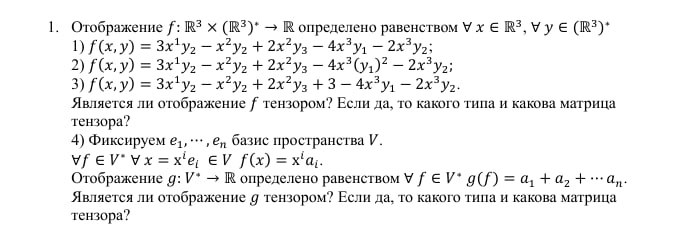
\includegraphics{assets/practice-2-task-1.jpg}
\end{center}

(Мне стало лень перепечатывать)

\textbf{Решение:}

Так ну давайте быстренько
\begin{enumerate}
    \item Да. $f \in T(3,3)$. Матрица тензора находится подстановкой базисных векторов, сами посчитаете, дорогие читатели.
    \item Нет, тк есть $(y_1)^2$ и ломается линейность.
    \item Нет, тк есть $3$ и ломается линейность.
    \item Нет, тк мы изначально фиксируем базис для работы этой функции!!!
\end{enumerate}

\subsubsection{Задание 2.}

$\dim V = 3, D$ - 3-форма на пространстве $V$ такая, что $D(e_1,e_2,e_3) = 1$, где $e_1,e_2,e_3$ - базис пространства $V$.
\begin{enumerate}
    \item Определить тип тензора $D$ и составить его матрицу
    \item Записать матрицу любой другой три формы на пространстве $V$
    \item выписать формулу для значения $D$ на наборе векторов $a,b,c$ пространства $V$
\end{enumerate}

\textbf{Решение:}

$D \in T(3,0)$. Ну начнем с того, что у нас $D$ - форма антисимметрична, то есть значения  при совпадающих индексах $i,j,k$ будут нулями. Зная это составим матрицу и получим:
$$\begin{pmatrix}[ccc|ccc|ccc]
    0 & 0 & 0 & 0 & 0 & -1 & 0& 1& 0 \\
    0 & 0 & 1 & 0 & 0 & 0 & -1 & 0 & 0 \\
    0 & -1 & 0 & 1 & 0 & 0 & 0 & 0 & 0 \\
\end{pmatrix}$$
Если мы хотим получить любую такую матрицу, то нам надо будет лишь подставить $\alpha$ - значение на базисных векторах:
$$\begin{pmatrix}[ccc|ccc|ccc]
    0 & 0 & 0 & 0 & 0 & -\alpha & 0& \alpha& 0 \\
    0 & 0 & \alpha & 0 & 0 & 0 & -\alpha & 0 & 0 \\
    0 & -\alpha & 0 & \alpha & 0 & 0 & 0 & 0 & 0 \\
\end{pmatrix}$$
Выписать формулу тривиально, тк это будет просто определитель матрицы.

\subsubsection{Задание 3.}

Записать формулу замены координат для тензора ранга 2 в матричном виде.

\textbf{Решение:}

У нас есть три случая:
\begin{enumerate}
    \item $\alpha^{ij} \in T(0,2)$.
    $$\alpha'^{\,kl}= \alpha^{ij} s^{k} _i s^l_j = (S\alpha S^T)^k_l$$
    \item $\alpha^{i}_j \in T(1,1)$.
     $$a'^k_l = \alpha^i_j t^j_l s^k_i= (\alpha^i_j t_l^j)s_i^k = (\alpha T)^i_l s^k_i = (S\alpha T)^k_l$$
    \item $\alpha^{}_{ij} \in T(2,0)$. 
    $$\alpha'_{kl} =\alpha_{ij}t_k^i t_l^j=(T^T \alpha T)^k_l$$
\end{enumerate}

\subsubsection{Задание 4.}

Тензор $\alpha \in T(2,1)$ задан матрицей своих координат
$$\begin{pmatrix}
    1 &3 & 2 &4 & 5 &6 & 7 & 8 & 9 \\
    4 &3&2 &1 &5 & 9 & 8 & 7  & 6\\
    9 & 8 & 7 & 6  & 5 & 4 &3 & 2 &1
\end{pmatrix}$$
Вычислить элемент матрицы тензора $\alpha'^{\, 2}_{13}$ в новом базисе $e_1' = e_1,e_2' = e_3, e_3'=e_2$.

\textbf{Решение:}

Ну тут все легко, ведь просто поменяли местами  2 вектора. То есть на самом деле
$\alpha'^{\, 2}_{13} = \alpha^3_{12} = 6$

\subsubsection{Задание 5.}

Найти тип и матрицу тензора $\gamma = \alpha \otimes \beta$ и $\overline{\gamma} = \beta \otimes \alpha$, где $\alpha$ и $\beta$ заданы соответственно своими матрицами.
\begin{enumerate}
    \item $\alpha \in T(0,1), \alpha = \begin{pmatrix}
        1 \\
        -1\\ 
        0
    \end{pmatrix}, \beta \in T(2,0), \beta = \begin{pmatrix}
        1 & 2 & 3\\
        4 & 5 & 6\\
        7 & 8 & 9\\
    \end{pmatrix}$
    \item $\alpha \in T(0,1),\alpha = \begin{pmatrix}
        1 \\
        -1\\ 
        0
    \end{pmatrix}, \beta \in T(1,1), \beta = \begin{pmatrix}
        1 & 2 & 3\\
        4 & 5 & 6\\
        7 & 8 & 9\\
    \end{pmatrix}$
\end{enumerate}
\textbf{Решение:}

Решим сначала первый случай. Заметим, что в данном случае $\gamma = \overline{\gamma}$. И будем делать все по формуле:
$$\gamma^i_{jk} = \begin{pmatrix}[ccc|ccc|ccc]
    1 & 4 & 7 & 2 & 5 & 8 & 3 & 6 & 9\\
    -1 & -4 & -7 & -2 &-5 &-8 & -3&-6&-9\\
    0 & 0&0&0&0&0&0&0&0
\end{pmatrix}$$
Теперь второй пункт:
$$\gamma^{ij}_k = \alpha^i \cdot \beta^j_k =\begin{pmatrix}[ccc|ccc|ccc]
    1 & 4 & 7 & 2 & 5 & 8 & 3 & 6 & 9\\
    -1 & -4 & -7 & -2 &-5 &-8 & -3&-6&-9\\
    0 & 0&0&0&0&0&0&0&0
\end{pmatrix}$$
$$\overline{\gamma}^{ij}_k =\beta^i_k\cdot \alpha^j =  \begin{pmatrix}[ccc|ccc|ccc]
    1 & -1 & 0 & 2 & -2 & 0 & 3 &-3&0\\
    4 & -4 & 0 & 5 & -5 & 0 & 6&-6&0\\
    7&-7&0&8&-8&0&9&-9&0
\end{pmatrix} $$

\subsubsection{Задание 6.}

\begin{center}
   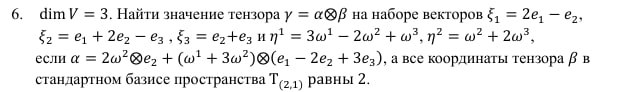
\includegraphics{assets/practice-2-task-6.jpg}
\end{center}

\textbf{Решение:}

Для этого, я должен раскидать $\xi,\eta$ между $a,b$. $a\in T(1,1)$, $b\in T(2,1)$. Жестко раскидываем векторочки по функциональному свойству и выиграли.


\subsubsection{Задание 7.}

$\alpha \in T(1,1), x \in T(0,1), \gamma = \alpha \otimes x$

Написать две возможные свертки.

\textbf{Решение:}

просто в тупую



